\documentclass[9pt]{IEEEtran}

\usepackage[english]{babel}
\usepackage{graphicx}
\usepackage{epstopdf}
\usepackage{fancyhdr}
\usepackage{amsmath}
\usepackage{amsthm}
\usepackage{amssymb}
\usepackage{url}
\usepackage{array}
\usepackage{textcomp}
\usepackage{listings}
\usepackage{hyperref}
\usepackage{xcolor}
\usepackage{colortbl}
\usepackage{float}
\usepackage{gensymb}
\usepackage{longtable}
\usepackage{supertabular}
\usepackage{multicol}

\usepackage[utf8x]{inputenc}

\usepackage[T1]{fontenc}
\usepackage{lmodern}
\input{glyphtounicode}
\pdfgentounicode=1

\graphicspath{{./figures/}}
\DeclareGraphicsExtensions{.pdf,.png,.jpg,.eps}

% correct bad hyphenation here
\hyphenation{op-tical net-works semi-conduc-tor trig-gs}

% ============================================================================================

\title{\vspace{0ex}
Exercise 1: Optical flow}

\author{Ilija Tavchioski\vspace{-4.0ex}}

% ============================================================================================

\begin{document}

\maketitle

\section{Introduction}
Optical flow is an important information when it comes to tracking a moving objects in a video. In this assignment the goal is to implement two well known algorithms for calculating the optical flow of each pixel.
The first one is Lucas-Kanade and the second one is Horn-Schunck method, and the research goal of this project is to compare their results on several examples, explain their hyper-parameters and experiment with possible improvements and research their anomalies.

\section{Experiments}
\subsection{Implementation}
\subsection{Results}
\begin{figure}[h]
    \centering
    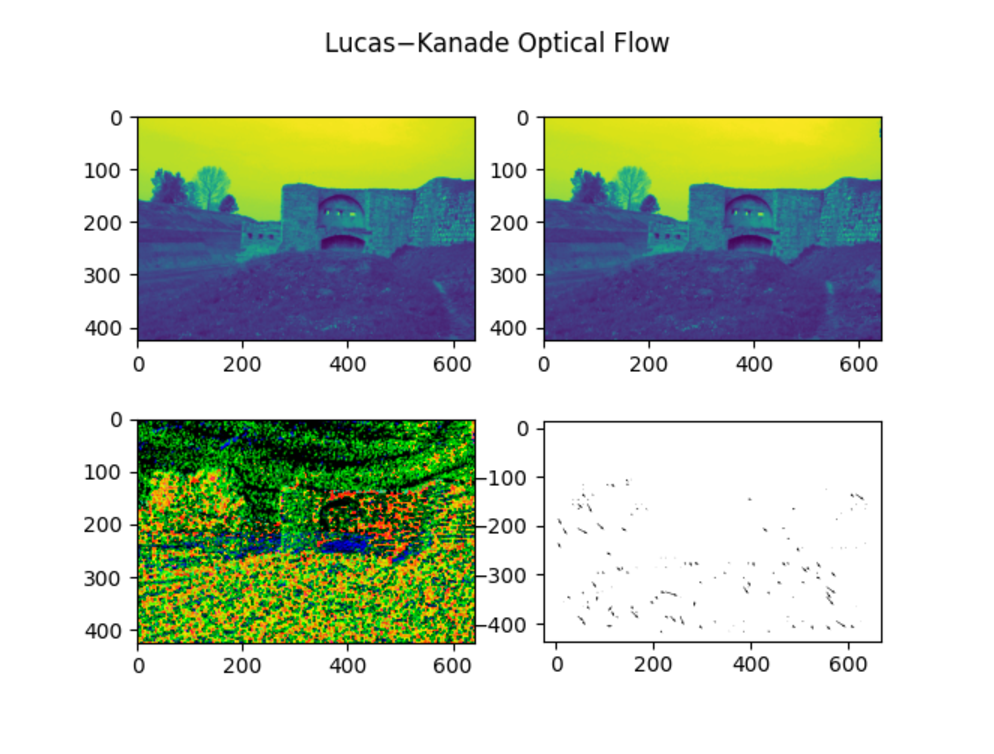
\includegraphics[width=1\columnwidth]{collisionlk.eps}
    \label{fig:disparitylk}
\end{figure}
\begin{figure}[h]
    \centering
    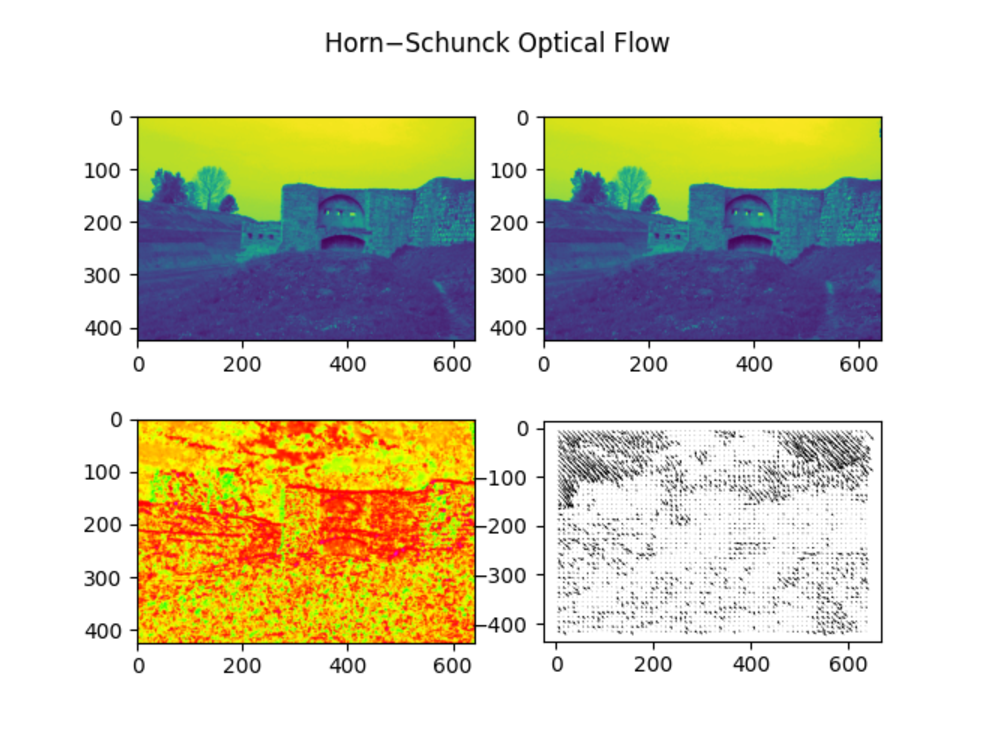
\includegraphics[width=1\columnwidth]{collisionhs.eps}
    \label{fig:disparityhs}
\end{figure}

\begin{figure}[h]
    \centering
    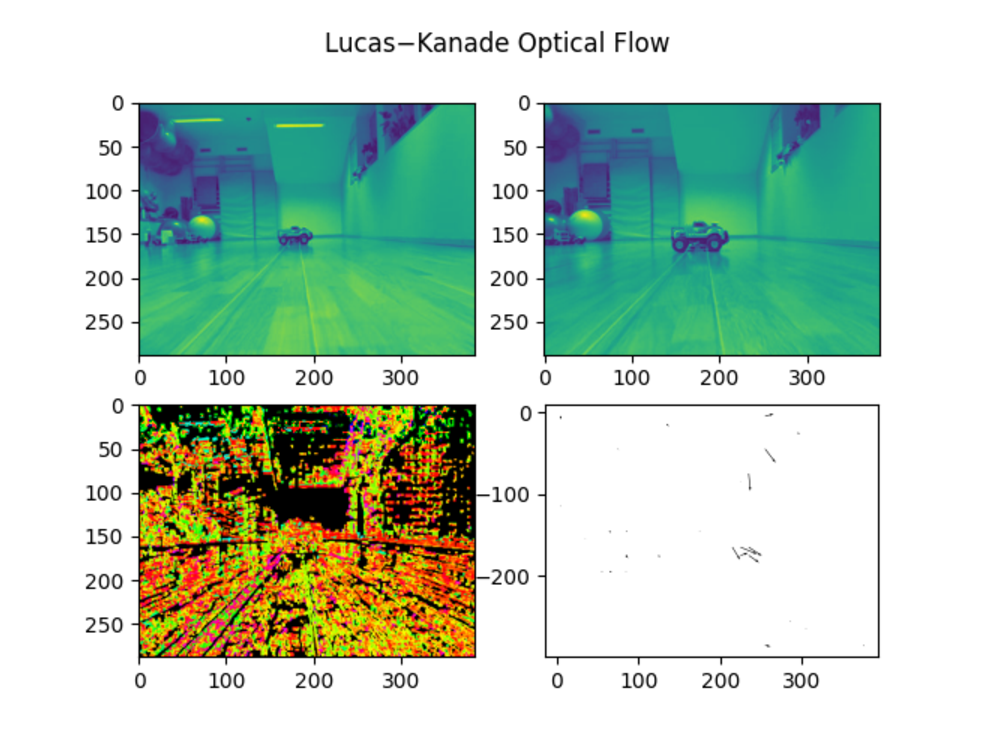
\includegraphics[width=1\columnwidth]{disparitylk.eps}
    \label{fig:collisionlk}
\end{figure}
\begin{figure}[h]
    \centering
    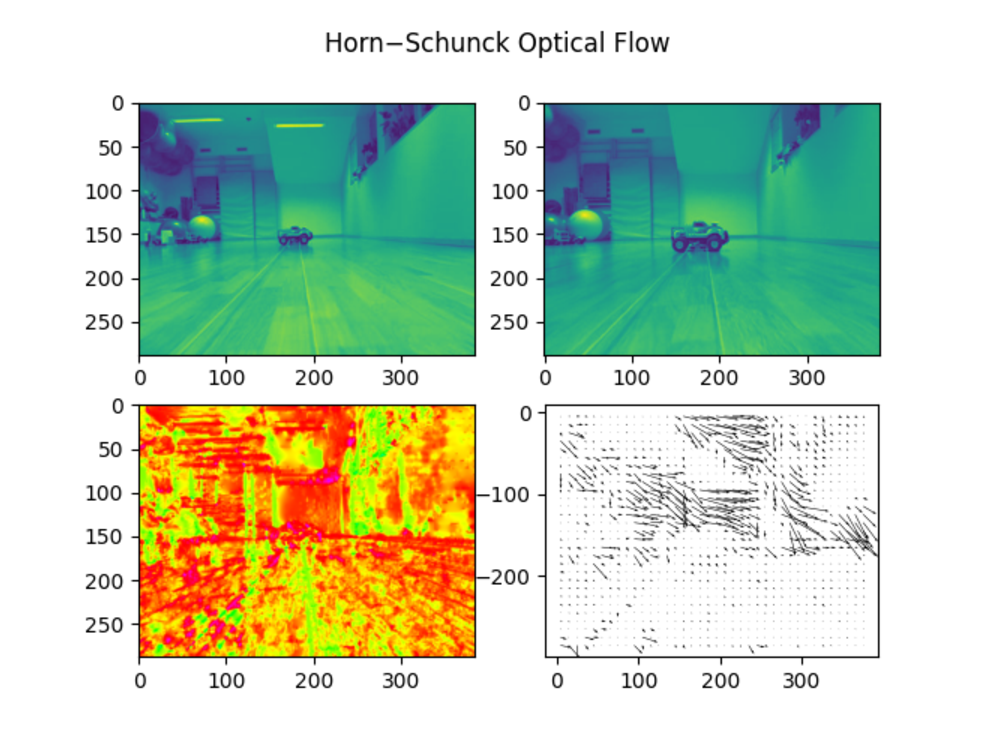
\includegraphics[width=1\columnwidth]{disparityhs.eps}
    \label{fig:collisionhs}
\end{figure}

\begin{figure}[h]
    \centering
    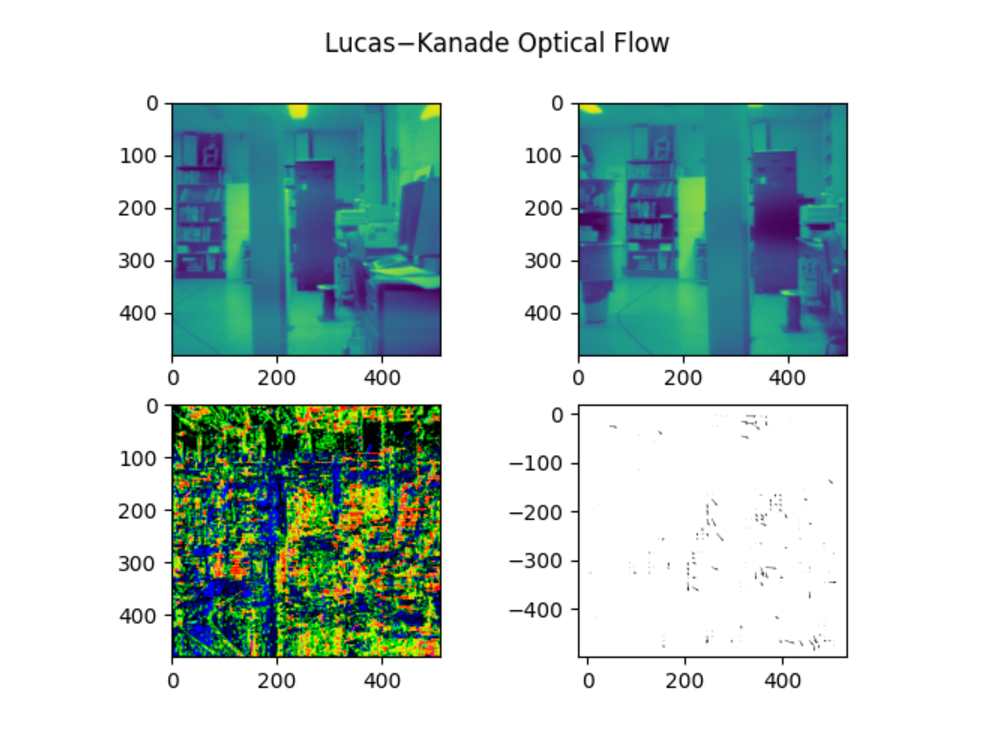
\includegraphics[width=1\columnwidth]{lab2lk.eps}
    \label{fig:lab2lk}
\end{figure}
\begin{figure}[h]
    \centering
    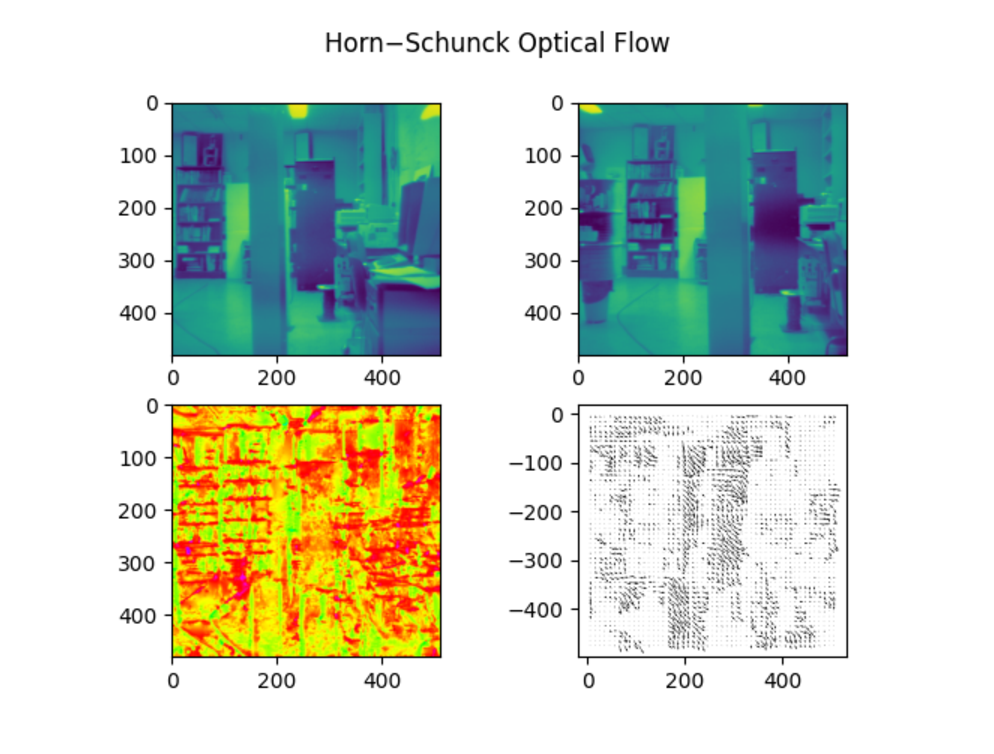
\includegraphics[width=1\columnwidth, scale=0.5]{lab2hs.eps}
    \label{fig:lab2hs}
\end{figure}

As we can see in our results (see Fig. \ref{fig:lab2hs} \ref{fig:lab2lk} \ref{fig:collisionlk} \ref{fig:collisionhs} \ref{fig:disparitylk} \ref{fig:disparityhs}), the Horn-Schunck algorithm is better in determing the flow in comparison to Lucas-Kanade which barely determine the flow due to several reasons such us when the determinant of matrix is 0 and we have unreliable result of 0 vector in direction.
This can be see especially in Fig. \ref{fig:collisionlk} when the position of the object in the two frames is drastic.
\subsection{Rliability of Lucas-Kanade optical flow}
\subsection{Parameters of the methods}
The methods have the following parameters, $\sigma$ which is the standard deviation of the gaussian kernel this parameter does not makes much of a difference of course it still need be in the range of (1, 6) since if it is too high will disrupt the image and if it is too low won't have any implication, $N$ which is the size of the neighbourhood. these two parameters are only for the Lucas-Kanade algorithm, this parameter especially if the frames are more moving needs to be higher \ref{fig:lab2lk7} in order to catch moving of the pixel in wider neightbourhood, but if it is too high will give a wrong result, the optimal number is around (3, 7).
\begin{figure}[h]
    \centering
    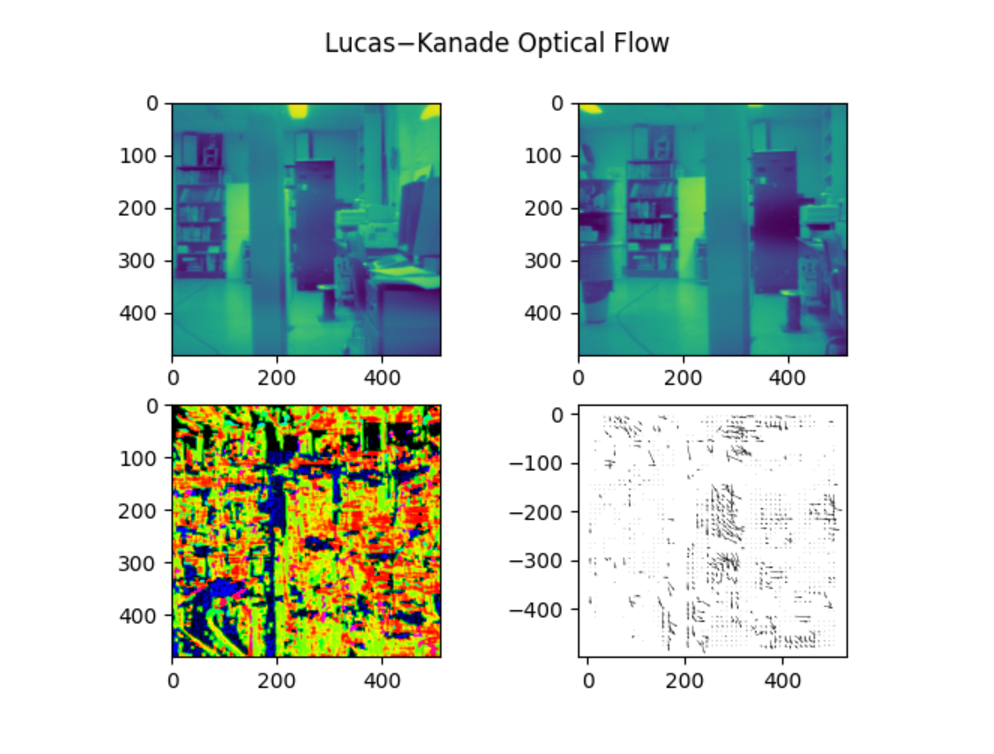
\includegraphics[width=1\columnwidth, scale=0.5]{lab2lk7.eps}
    \label{fig:lab2lk7}
\end{figure}
For the Horn-Schunck algorithm we have the number of iterations, which if it is low the directions will be not accurate and as the N is higher the directions are more accurate until convergence the optimal number is around 1000.
Another parameter is $\lambda$ which is the regularization cost. Larger values of $\lambda$ lead to smoother flow.
\subsection{Optimization}
\subsection{Pyramidal Lucas-Kanade}

\section{Conclusion}


\bibliographystyle{IEEEtran}
\bibliography{bibliography}

\end{document}
